% questions.tex —— 2009 年·普通高等学校招生考试·重庆卷·理科 · 题目内容片段（无答案）
% 由 tools/generate_projects.py 依来源总账自 2009/2009_数学真题_重庆理_试题.md 生成，勿手改（改源 MD 后重跑）


状态：needs-review；依固定候选 PDF 两页（印刷页 503–504）逐题核验，两幅图已矢量重绘。原页未印分值，不补。

\gkpart{一、选择题}

\begin{question}
\gkti{1}直线 $y=x+1$ 与圆 $x^2+y^2=1$ 的位置关系是（　）

（A）相切

（B）相交但直线不过圆心

（C）直线过圆心

（D）相离

\end{question}
\begin{question}
\gkti{2}已知复数 $z$ 的实部为 $-1$，虚部为 $2$，则 $\dfrac{5i}{z}=$（　）

（A）$2-i$

（B）$2+i$

（C）$-2-i$

（D）$-2+i$

\end{question}
\begin{question}
\gkti{3}$\left(x^2+\dfrac2x\right)^8$ 的展开式中 $x^4$ 的系数是（　）

（A）$16$

（B）$70$

（C）$560$

（D）$1120$

\end{question}
\begin{question}
\gkti{4}已知 $|\boldsymbol a|=1$，$|\boldsymbol b|=6$，$\boldsymbol a\cdot(\boldsymbol b-\boldsymbol a)=2$，则向量 $\boldsymbol a$ 与 $\boldsymbol b$ 的夹角是（　）

（A）$\dfrac\pi6$

（B）$\dfrac\pi4$

（C）$\dfrac\pi3$

（D）$\dfrac\pi2$

\end{question}
\begin{question}
\gkti{5}不等式 $|x+3|-|x-1|\leqslant a^2-3a$ 对任意实数 $x$ 恒成立，则实数 $a$ 的取值范围为（　）

（A）$(-\infty,-1]\cup[4,+\infty)$

（B）$(-\infty,-2]\cup[5,+\infty)$

（C）$[1,2]$

（D）$(-\infty,1]\cup[2,+\infty)$

\end{question}
\begin{question}
\gkti{6}锅中煮有芝麻馅汤圆 $6$ 个，花生馅汤圆 $5$ 个，豆沙馅汤圆 $4$ 个，这三种汤圆的外部特征完全相同．从中任意舀取 $4$ 个汤圆，则每种汤圆都至少取到 $1$ 个的概率为（　）

（A）$\dfrac8{91}$

（B）$\dfrac{25}{91}$

（C）$\dfrac{48}{91}$

（D）$\dfrac{60}{91}$

\end{question}
\begin{question}
\gkti{7}设 $\triangle ABC$ 的三个内角 $A$，$B$，$C$，向量 $\boldsymbol m=(\sqrt3\sin A,\sin B)$，$\boldsymbol n=(\cos B,\sqrt3\cos A)$，若 $\boldsymbol m\cdot\boldsymbol n=1+\cos(A+B)$，则 $C=$（　）

（A）$\dfrac\pi6$

（B）$\dfrac\pi3$

（C）$\dfrac{2\pi}3$

（D）$\dfrac{5\pi}6$

\end{question}
\begin{question}
\gkti{8}已知 $\lim\limits_{x\to\infty}\left(\dfrac{2x^2}{x+1}-ax-b\right)=2$，其中 $a,b\in\mathbf R$，则 $a-b$ 的值为（　）

（A）$-6$

（B）$-2$

（C）$2$

（D）$6$

\end{question}
\begin{question}
\gkti{9}已知二面角 $\alpha-l-\beta$ 的大小为 $50^\circ$，$P$ 为空间中任意一点，则过点 $P$ 且与平面 $\alpha$ 和平面 $\beta$ 所成的角都是 $25^\circ$ 的直线的条数为（　）

（A）$2$

（B）$3$

（C）$4$

（D）$5$

\end{question}
\begin{question}
\gkti{10}已知以 $T=4$ 为周期的函数

\nopagebreak[4]
\[f(x)=\begin{cases}m\sqrt{1-x^2},&x\in(-1,1],\\ 1-|x-2|,&x\in(1,3],\end{cases}\]

其中 $m>0$．若方程 $3f(x)=x$ 恰有 $5$ 个实数解，则 $m$ 的取值范围为（　）

（A）$\left(\dfrac{\sqrt{15}}3,\dfrac83\right)$

（B）$\left(\dfrac{\sqrt{15}}3,\sqrt7\right)$

（C）$\left(\dfrac43,\dfrac83\right)$

（D）$\left(\dfrac43,\sqrt7\right)$

\end{question}
\gkpart{二、填空题}

\begin{question}
\gkti{11}若 $A=\{x\in\mathbf R\mid |x|<3\}$，$B=\{x\in\mathbf R\mid 2^x>1\}$，则 $A\cap B=$ $\underline{\qquad}$．

\end{question}
\begin{question}
\gkti{12}若 $f(x)=\dfrac1{2^x-1}+a$ 是奇函数，则 $a=$ $\underline{\qquad}$．

\end{question}
\begin{question}
\gkti{13}将 $4$ 名大学生分配到 $3$ 个乡镇去当村官，每个乡镇至少一名，则不同的分配方案有$\underline{\qquad}$种．（用数字作答）

\end{question}
\begin{question}
\gkti{14}设 $a_1=2$，$a_{n+1}=\dfrac2{a_n+1}$，$b_n=\dfrac{a_n+2}{a_n-1}$，$n\in\mathbf N^*$，则数列 $\{b_n\}$ 的通项 $b_n=$ $\underline{\qquad}$．

\end{question}
\begin{question}
\gkti{15}已知双曲线 $\dfrac{x^2}{a^2}-\dfrac{y^2}{b^2}=1$（$a>0$，$b>0$）的左、右焦点分别为 $F_1(-c,0)$，$F_2(c,0)$．若双曲线上存在一点 $P$ 使 $\dfrac{\sin\angle PF_1F_2}{\sin\angle PF_2F_1}=\dfrac ac$，则该双曲线的离心率的取值范围为$\underline{\qquad}$．

\end{question}
\gkpart{三、解答题}

\begin{question}
\gkti{16}设函数 $f(x)=\sin\left(\dfrac\pi4x-\dfrac\pi6\right)-2\cos^2\dfrac\pi8x+1$．

（1）求 $f(x)$ 的最小正周期；

（2）若函数 $y=g(x)$ 与 $y=f(x)$ 的图象关于直线 $x=1$ 对称，求当 $x\in\left[0,\dfrac43\right]$ 时 $y=g(x)$ 的最大值．

\end{question}
\begin{question}
\gkti{17}某单位为绿化环境，移栽了甲、乙两种大树各 $2$ 株．设甲、乙两种大树移栽的成活率分别为 $\dfrac23$ 和 $\dfrac12$，且各株大树是否成活互不影响．求移栽的 $4$ 株大树中：

（1）两种大树各成活 $1$ 株的概率；

（2）成活的株数 $\xi$ 的分布列与期望．

\end{question}
\begingroup
\renewenvironment{question}{\Needspace{0.5\textheight}}{}
\begin{question}
\gkti{18}设函数 $f(x)=ax^2+bx+k$（$k>0$）在 $x=0$ 处取得极值，且曲线 $y=f(x)$ 在点 $(1,f(1))$ 处的切线垂直于直线 $x+2y+1=0$．

（1）求 $a$，$b$ 的值；

（2）若函数 $g(x)=\dfrac{\mathrm e^x}{f(x)}$，讨论 $g(x)$ 的单调性．

\Needspace{0.4\textheight}
\end{question}
\endgroup
\begin{question}
\gkti{19}如图，在四棱锥 $S-ABCD$ 中，$AD\parallel BC$ 且 $AD\perp CD$；平面 $CSD\perp$ 平面 $ABCD$，$CS\perp DS$，$CS=2AD=2$，$E$ 为 $BS$ 的中点，$CE=\sqrt2$，$AS=\sqrt3$．求：

（1）点 $A$ 到平面 $BCS$ 的距离；

（2）二面角 $E-CD-A$ 的大小．
\nopagebreak[4]
\begin{center}% 2009 年重庆卷理科第 19 题：四棱锥 S-ABCD，E 为 BS 中点。
% 来源 PDF：普通高考/2009/2009重庆理.pdf，SHA-256 6a815fa472e380a3f1143e8cdd93712e142309acb7a95176783499406a8e15f1。
% 原页：第 2 页（A3 三栏）第 1 栏上部，书页码 504。
% 重绘依据：由题设取 D(0,0,0)、C(√6,0,0)、A(0,1,0)、B(√6,2,0)、S(√6/3,0,2/√3)。
%   投影取 (x,y,z) -> (x+0.35y, -1.2z+0.25y)，使 S 在下方、B 在上方，与原页视角一致。
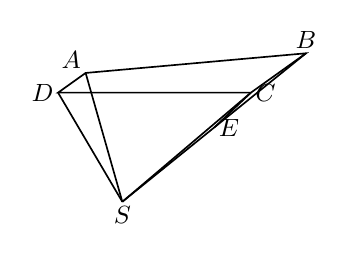
\begin{tikzpicture}[semithick, every node/.style={inner sep=1.4pt, font=\small}]
  \coordinate (D) at (0.000,0.000);
  \coordinate (C) at (2.449,0.000);
  \coordinate (A) at (0.350,0.250);
  \coordinate (B) at (3.149,0.500);
  \coordinate (S) at (0.816,-1.386);
  \coordinate (E) at (1.983,-0.443);

  % 底面
  \draw (A) -- (B) -- (C) -- (D) -- cycle;
  % 侧棱
  \draw (S) -- (D);
  \draw (S) -- (C);
  \draw (S) -- (A);
  \draw (S) -- (B);
  % CE
  \draw (C) -- (E);

  % 标注
  \node[left] at (D) {$D$};
  \node[right] at (C) {$C$};
  \node[above left] at (A) {$A$};
  \node[above] at (B) {$B$};
  \node[below] at (S) {$S$};
  \node[right] at (E) {$E$};
\end{tikzpicture}
\end{center}
\nopagebreak[4]
\Needspace{0.4\textheight}
\end{question}
\begingroup
\renewenvironment{question}{\Needspace{0.5\textheight}}{}
\begin{question}
\gkti{20}已知以原点 $O$ 为中心的椭圆的一条准线方程为 $x=\dfrac{4\sqrt3}3$，离心率 $e=\dfrac{\sqrt3}2$，$M$ 是椭圆上的动点．

（1）若点 $C$，$D$ 的坐标分别是 $(0,-\sqrt3)$，$(0,\sqrt3)$，求 $|MC|\cdot|MD|$ 的最大值；

（2）如图，点 $A$ 的坐标为 $(1,0)$，$B$ 是圆 $x^2+y^2=1$ 上的点，$N$ 是点 $M$ 在 $x$ 轴上的射影，点 $Q$ 满足条件：$\overrightarrow{OQ}=\overrightarrow{OM}+\overrightarrow{ON}$，$\overrightarrow{QA}\cdot\overrightarrow{BA}=0$．求线段 $QB$ 的中点 $P$ 的轨迹方程．
\nopagebreak[4]
\begin{center}% 2009 年重庆卷理科第 20 题：椭圆 x^2+y^2/4=1、单位圆与点 A、B、M、N、Q。
% 来源 PDF：普通高考/2009/2009重庆理.pdf，SHA-256 6a815fa472e380a3f1143e8cdd93712e142309acb7a95176783499406a8e15f1。
% 原页：第 2 页（A3 三栏）第 2 栏中部，书页码 504。
% 重绘依据：按更正后的椭圆 x^2+y^2/4=1 绘制；取 M(0.8,1.2)、N(0.8,0)、Q(1.6,1.2)，
%   B 取单位圆上满足 QA⊥BA 的点 (-0.6,0.8)，仅作示意。
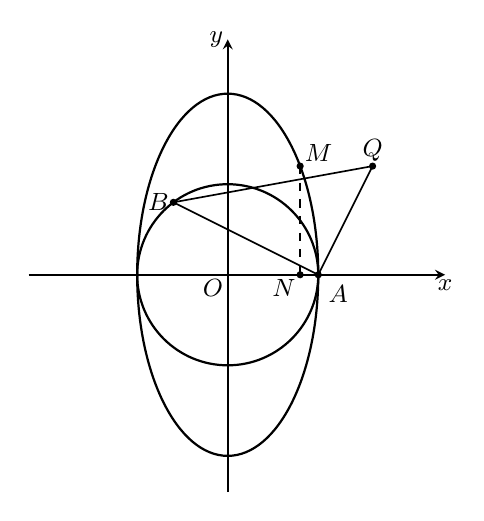
\begin{tikzpicture}[semithick, x=1.15cm, y=1.15cm, every node/.style={inner sep=1.4pt, font=\small}]
  % 坐标轴
  \draw[-stealth] (-2.2,0) -- (2.4,0) node[below] {$x$};
  \draw[-stealth] (0,-2.4) -- (0,2.6) node[left] {$y$};
  \node[below left] at (0,0) {$O$};

  % 椭圆
  \draw[thick] (0,0) ellipse (1 and 2);
  % 单位圆
  \draw[thick] (0,0) circle (1);

  % 点
  \coordinate (A) at (1.0,0.0);
  \coordinate (M) at (0.8,1.2);
  \coordinate (N) at (0.8,0.0);
  \coordinate (Q) at (1.6,1.2);
  \coordinate (B) at (-0.6,0.8);
  \fill (A) circle (1.3pt);
  \fill (M) circle (1.3pt);
  \fill (N) circle (1.3pt);
  \fill (Q) circle (1.3pt);
  \fill (B) circle (1.3pt);

  % 辅助线
  \draw[dashed] (M) -- (N);
  \draw (Q) -- (B);
  \draw (Q) -- (A);
  \draw (A) -- (B);

  % 标注
  \node[below right=2pt] at (A) {$A$};
  \node[above right] at (M) {$M$};
  \node[below left] at (N) {$N$};
  \node[above] at (Q) {$Q$};
  \node[left] at (B) {$B$};
\end{tikzpicture}
\end{center}
\nopagebreak[4]
\end{question}
\endgroup
\begin{question}
\gkti{21}设 $m$ 个不全相等的正数 $a_1,a_2,\cdots,a_m$（$m\geqslant7$）依次围成一个圆圈．

（1）若 $m=2009$，且 $a_1,a_2,\cdots,a_{1005}$ 是公差为 $d$ 的等差数列，而 $a_1,a_{2009},a_{2008},\cdots,a_{1006}$ 是公比为 $q=d$ 的等比数列；数列 $a_1,a_2,\cdots,a_m$ 的前 $n$ 项和 $S_n$（$n\leqslant m$）满足：$S_3=15$，$S_{2009}=S_{2007}+12a_1$，求通项 $a_n$（$n\leqslant m$）；

\Needspace{5\baselineskip}
（2）若每个数 $a_n$（$n\leqslant m$）是其左右相邻两数平方的等比中项，求证：

\nopagebreak[4]
\[a_1+\cdots+a_6+a_7^2+\cdots+a_m^2>ma_1a_2\cdots a_m.\]

\end{question}